
%(BEGIN_QUESTION)
% Copyright 2010, Tony R. Kuphaldt, released under the Creative Commons Attribution License (v 1.0)
% This means you may do almost anything with this work of mine, so long as you give me proper credit

An inventor claims to have made an ``over-unity'' machine that outputs more electrical power than it inputs.  It consists of a three-phase AC electric motor with its shaft directly coupled to a DC generator.  A resistive load is connected to the DC generator's output for testing and demonstration purposes.  In use, the point is to power real electrical loads from the DC generator's output, using less AC power from the power company than if equivalent loads were run directly off AC line power:

$$\includegraphics[width=15.5cm]{i02397x01.eps}$$

The inventor takes the following measurements and makes the following calculations, then declares the machine to be more than 100\% efficient:

\begin{itemize}
\item{} AC line voltage (motor, measured) = 476.5 volts RMS
\item{} AC line current (motor, measured) = 12.7 amps RMS
\item{} $P_{input}$ (calculated) = 6.052 kW
\vskip 10pt
\item{} DC line voltage (generator, measured) = 231 volts DC
\item{} DC line current (generator, measured) = 37.8 amps DC
\item{} $P_{output}$ (calculated) = 8.732 kW
\vskip 10pt
\item{} Efficiency ($P_{output} \over P_{input}$, calculated) = {\bf 144.3\%}
\end{itemize}

\vskip 10pt

Explain why this inventor's claim is false, and calculate the true efficiency of the system.

\underbar{file i02397}
%(END_QUESTION)





%(BEGIN_ANSWER)

Over-unity machines are impossible, because they would violate the {\it Law of Energy Conservation}.  The inventor's mistake here was to neglect to include the $\sqrt{3}$ factor in calculating input power.  Had he did so, his calculated efficiency would have been only 83.31\%.

%(END_ANSWER)





%(BEGIN_NOTES)

{\bf This question is intended for exams only and not worksheets!}.

%(END_NOTES)

